\newif\ifanonymous\anonymousfalse
\newif\ifspringer\springertrue
\newif\iffinal\finalfalse

\ifspringer
  \documentclass[a4paper]{llncs}
\else
  \ifanonymous
    \documentclass[journal=tosc,submission]{iacrtrans}
  \else
    \iffinal
      \documentclass[journal=tosc,final]{iacrtrans}
    \else
      \documentclass[journal=tosc,preprint]{iacrtrans}
    \fi
  \fi
\fi

%%% packages %%%
\usepackage{tikz}
%\usetikzlibrary{calc,cipher}
%\usepackage{booktabs,multirow}
%\usepackage{subcaption}
%\usepackage[color=blue!30]{todonotes}

%%%%%%%%%%%%%%%%%%%%%%%%%%%%%%%%%
\usepackage{subcaption}
\usepackage{amsmath}
\usepackage{amssymb}
\usepackage{mathtools}
\usepackage[linesnumbered,ruled,lined]{algorithm2e}
%\usepackage{algorithmicx}
\usepackage{algpseudocode}
\usepackage[flushleft]{threeparttable}
\usepackage{xcolor}
\newcommand\mycommfont[1]{\small\ttfamily\textcolor{blue}{#1}}
\SetCommentSty{mycommfont}
\usepackage{comment}
%%%%%%%%%%%%%%%%%%%%%%%%%%%%%%%%%%

\ifspringer
  \usepackage{amsmath}
  \usepackage[hidelinks]{hyperref}
  \AtBeginDocument{\def\doi#1{\url{https://doi.org/#1}}}
  \def\figureautorefname{Figure}%
  \def\tableautorefname{Table}%
  \def\appendixautorefname{Appendix}%
  \def\sectionautorefname{Section}%
  \def\subsectionautorefname{Section}%
  \def\subsubsectionautorefname{Section}%
  \renewcommand{\tabcolsep}{4pt}%
\fi

\iffinal\else
  \usepackage{orcidlink}
  \let\orcidID\orcidlink
\fi

%%% macros %%%


%%% metadata %%%
\ifanonymous\else
\author{%
       Akram Khalesi\inst{1}\orcidID{0000-0000-0000-0000}
  \and Zahra Ahmadian\inst{1}\orcidID{0000-0000-0000-0000}
  \and Hosein Hadipour\inst{1}\orcidID{0000-0002-3820-3765}
  \and ... %\inst{1,2}
}
\institute{
  Ruhr University Bochum \\
  \email{mtest@gmail.com},
  \email{test@gmail.comt},
  \email{hsn.hadipour@gmail.com}
  % \and
  %...
}
\fi

\title{Paper Title}
%\title[short]{Paper Title} % iacrtrans only
%\subtitle{...} % iacrtrans only

\newcommand{\thekeywords}{Cryptanalysis \and ...}

\begin{document}
\ifspringer\else\iffinal
  \setfirstpage{1}
\setlastpage{0}
\setvolume{2022}
\setnumber{2}

\setISSN{2519-173X}
\makeatletter
\setDOI{10.46586/tosc.v\IACR@vol.i\IACR@no.\IACR@fp-\IACR@lp}
\makeatother

\fi\fi


\maketitle

\ifspringer \pagestyle{plain} \else \keywords{\protect\thekeywords} \fi

\begin{abstract}
  ...

  \ifspringer \keywords{\protect\thekeywords} \fi
\end{abstract}


%%% INTRODUCTION %%%%%%%%%%%%%%%%%%%%%%%%%%%%%%%%%%%%%%%%%%%%%%%%%%%%%%%
\section{Introduction}\label{sec:introduction}

...

\section{Preliminaries}
\subsection{Notation}
\subsection{integral Attack}
\subsection{Brief Introduction of CHILOW-(32+$\tau$)}
\section{Integral Cryptanalysis of CHILOW-(32+$\tau$)}

\subsection{Search for Integral Distinguishers}
We have exhaustively searched for all possible 3-round integral distinguishers involving four active bits and identified 9 such distinguishers, each resulting in 32 balanced bits. These distinguishers are given by:
\begin{equation*}
\begin{split}
\{5,7,9,11\}\xrightarrow{3-round}\{0,...,31\}, \\
\{6,8,10,12\}\xrightarrow{3-round}\{0,...,31\}, \\
\{7,9,11,14\}\xrightarrow{3-round}\{0,...,31\}, \\
\{8,10,12,14\}\xrightarrow{3-round}\{0,...,31\}, \\
\{14,17,19,21\}\xrightarrow{3-round}\{0,...,31\}, \\
\{21,23,25,27\}\xrightarrow{3-round}\{0,...,31\}, \\
\{22,24,26,28\}\xrightarrow{3-round}\{0,...,31\}, \\
\{23,25,27,29\}\xrightarrow{3-round}\{0,...,31\}, \\
\{23,25,27,30\}\xrightarrow{3-round}\{0,...,31\}.
\end{split}
\end{equation*}
Here, the sets on the left denote the indices of active input bits, while the set on the right represents the 32 output bits that are balanced after 3 rounds.

Similarly, we conducted a comprehensive search for all possible 3-round integral distinguishers involving three active bits. The maximum number of balanced bits observed is 5, which occurs in two cases. Additionally, we identified 10 distinguishers that result in 3 balanced bits. The most notable results are listed below:
\begin{equation*}
\begin{split}
\{21,23,25\}\xrightarrow{3-round}\{2,3,14,25,26\}, \\
\{27,29,31\}\xrightarrow{3-round}\{5,14,22,25,28\}, \\
\{3,5,7\}\xrightarrow{3-round}\{0,4,24\}, \\
\{6,8,10\}\xrightarrow{3-round}\{5,24,27\}, \\
\{7,9,11\}\xrightarrow{3-round}\{0,9,12\}, \\
\{9,11,13\}\xrightarrow{3-round}\{7,11,31\}, \\
\{12,14,17\}\xrightarrow{3-round}\{6,21,24\}, \\
\{17,19,21\}\xrightarrow{3-round}\{14,19,23\}, \\
\{18,20,22\}\xrightarrow{3-round}\{6,18,27\}, \\
\{19,21,25\}\xrightarrow{3-round}\{2,14,26\}, \\
\{22,24,26\}\xrightarrow{3-round}\{21,25,30\}, \\
\{26,28,30\}\xrightarrow{3-round}\{1,10,22\}.
\end{split}
\end{equation*}

\subsection{Key Recovery Attack on 6-round CHILOW-(32+$\tau$)}
\label{sec:6R-attack}

In this section, we introduce a key recovery attack on 6-round CHILOW-(32+$\tau$). The attack consists of four phases. \\

\textbf{First phase:} By employing 3-round integral distinguishers and extending them three rounds forward, we determine candidate values for the tweak states $T^{(4)}_{0,...,31}$, $T^{(5)}_{0,...,31}$ and $T^{(6)}_{0,...,31}$. The distinguishers used in this phase are:
\begin{equation*}
\begin{split}
\{21,23,25\}\xrightarrow{3-round}\{2,3,14,25,26\}, \texttt{ and}\\
\{21,23,25,27\}\xrightarrow{3-round}\{0,...,31\},
\end{split}
\end{equation*}
where the active bits in the first distinguisher form a subset of those in the second. This relationship is beneficial for reducing the number of required queries.

First, we choose three distinct sets of $2^{4}$ ciphertexts which are active in bit numbers $\{21,23,25,27\}$ and constant at other positions; and query for their corresponding plaintexts. Then, for $2^{96}$ possible values for $T^{(6)}_{0,...,31}||T^{(5)}_{0,...,31}||T^{(4)}_{0,...,31}$, we compute the parity of the third-round output for a subset of the first input set (according to the 3-round distinguisher with three active bits) and the values leading to the balanced property in bit numbers 2, 3, 14, 25, and 26 will be introduced as a candidate. We expect $2^{91}(=2^{96}\times 2^{-5})$ candidates on average with time comlexity $2^{98}(=2^{96}\times 2^{3}\times \frac{3}{6})$, due to the 5-bit condition corresponding to the 5-bit balanced property in the 96-bit guess. Afterward, for $2^{91}$ candidates for $T^{(6)}_{0,...,31}||T^{(5)}_{0,...,31}||T^{(4)}_{0,...,31}$, we compute the parrity of the entire first input set and reduce the number of candidates to $2^{64}=2^{91}\times2^{-(32-5)}$ with time complexity $2^{94}(=2^{91}\times 2^{4}\times \frac{3}{6})$, due to the expected 32-bit balanced property which 5 bits have already been exploited{\color{red}???}. For the candidate values for $T^{(6)}_{0,...,31}||T^{(5)}_{0,...,31}||T^{(4)}_{0,...,31}$, we also calculate the parity of the second and third input sets and reduce the number of candidates to one with time complexity $2^{67}(\approx ((2^{64}\times 2^{4})+(2^{32}\times 2^{4})) \times \frac{3}{6})$ encryptions, due to the $2\times 32$-bit condition. Hence, we get one candidate for $T^{(6)}_{0,...,31}||T^{(5)}_{0,...,31}||T^{(4)}_{0,...,31}$ on average, where the time complexity is dominated by $2^{98}+2^{94}$ encryptions and we estimate the total time complexity of this phase as $2^{98.1}$ encryptions.\\

\textbf{Second phase:} a 2-round integral distinguisher will be extended four rounds forward and for the candidate value for $T^{(6)}_{0,...,31}||T^{(5)}_{0,...,31}||T^{(4)}_{0,...,31}$ from the first phase, the parity will be checked for all $2^{32}$ possible values for $T^{(3)}_{0,...,31}$ and those leading to the balanced propoerty will be introduced as a candidate. The exploited distinguisher in this phase can be described as:
\begin{equation*}
\{21,23\}\xrightarrow{2-round}\{0,...,31\},
\end{equation*}
i.e., the input has 2 active bits, while the whole 32-bit output block is balanced. 

It should be noted that the active bits in the 2-round distinguisher is a subset of the active bits in the 3-round distinguisher. So, a subset of the chosen ciphertexts in the first phase could be used for the second phase, and no extra data is needed. 
We expect one $(=1\times 2^{32}\times 2^{-32})$ candidate on average for $T^{(6)}_{0,...,31}||T^{(5)}_{0,...,31}||T^{(4)}_{0,...,31}||T^{(3)}_{0,...,31}$, due to the 32-bit condition in the 32-bit guess for the candidate for $T^{(6)}_{0,...,31}||T^{(5)}_{0,...,31}||T^{(4)}_{0,...,31}$ from the first phase. Time complexity of this phase is estimated as $2^{34.5}(=2^{32}\times 2^{3} \times \frac{4}{6})$ encryptions.

\textbf{Third phase:} we test all $2^{96}$ possible values for $T^{(2)}_{0,...,31}||T^{(1)}_{0,...,31}||K_{64,...,95}$ with the candidate for $T^{(6)}_{0,...,31}||T^{(5)}_{0,...,31}||T^{(4)}_{0,...,31}||T^{(3)}_{0,...,31}$ from the previous phase on three distinct ciphertext-plaintext pairs to filter the contradictory guesses. In this phase, we expect one candidate for $T^{(6)}_{0,...,31}||T^{(5)}_{0,...,31}||T^{(4)}_{0,...,31}||T^{(3)}_{0,...,31}||T^{(2)}_{0,...,31}||T^{(1)}_{0,...,31}||K_{64,...,95}$ on average with time complexity $2^{97.6}(=2^{96}\times 3)$ decryptions. Since the data from the previous phases can be used, no extra data is required for this phase.

\textbf{Fourth phase:} note that $T^{(1)}$ depends only on the tweak $T$ and 64 bits of the master key $K_{0,...,63}$. Hence, for the value recovered for $T^{(1)}_{0,...,31}$ in the third phase, we guess $T^{(1)}_{32,...,63}$ and compute 64 bits of the master key as $K_{0,...,63}=\chi\!\!\!\chi_{64}^{-1}(L_{64}^{-1}(T^{(1)}))\oplus T$. This phase requires $2^{32}$ times $\chi\!\!\!\chi_{64}^{-1}(L_{64}^{-1}(.))$ operations. Considering $\chi\!\!\!\chi_{64}^{-1}(L_{64}^{-1}(.))$ operation as one-round encryption, we have $2^{32}$ candidates for $K_{0,...,95}$ with $2^{29.5}(=2^{32} \times \frac{1}{6})$ encryptions. {\color{red}(complexity of $\chi\!\!\!\chi_{64}^{-1}(L_{64}^{-1}(.))$ operation? is it possible?)} The memory required to restore these candidates for further investigation would be $2^{33.6}(\approx 2^{32}\times 3)$ 32-bit blocks which forms the memory complexity of the attack.

Afterward, we guess $K_{96,...,127}$ for each candidate value for $K_{0,...,95}$ and filter them by the values recovered for $T^{(i)}_{0,...,31}$ for $i\in \{2,3,4,5,6\}$. We expect to recover the master key with $2^{64}(=2^{32} \times 2^{32})$ decryptions at the end of this phase, since we guess 32-bit value for $K_{96,...,127}$ for $2^{32}$ candidates for $K_{0,...,95}$ and filter them by five 32-bit values.

\subsubsection{Complexity Analysis}
The attack requires $3\times 2^{4}$ chosen ciphertexts, and the overall data complexity is estimated as $2^{5.6}$ chosen ciphertexts. As shown in Table \ref{tab:6r-attack}, time complexity of the attack is dominated by $2^{98.1}$ encryptions in  phase 1 and $2^{97.6}$ decryptions in  phase 3. Consequently, the overall time complexity is estimated as $2^{98.9}$ encryptions. Finally, the memory complexity is $2^{33.6}$ 32-bit blocks, required during Phase 4.

\begin{table*}[t!]
\centering
\begin{center}
\caption{Summary of the key recovery attack on 6-round CHILOW-(32+$\tau$)}
\label{tab:6r-attack}
\renewcommand{\arraystretch}{1.5}
\scalebox{0.9}{
\begin{tabular}{cccc}
\hline
Phase & recovered paramerter & No. of candidates & Time complexity \\
\hline
1 & $T^{(6)}_{0,...,31}||T^{(5)}_{0,...,31}||T^{(4)}_{0,...,31}$ & 1 & $2^{98.1} enc$ \\
\hline
2 & $T^{(3)}_{0,...,31}$ & 1 & $2^{34.5}$ enc \\
\hline
3 & $T^{(2)}_{0,...,31}||T^{(1)}_{0,...,31}||K_{64,...,95}$ & 1 & $2^{97.6} dec$ \\
\hline
4 & $K_{0,...,63}||K_{96,...,127}$ & 1 & $2^{64} (dec) + 2^{29.5} (enc)$ \\
\hline
%5 & $K_{96,...,127}$ & 1 & $2^{64} dec$ \\
%\hline
\end{tabular}}
\end{center}
\end{table*}

\begin{figure*}
	\centering
	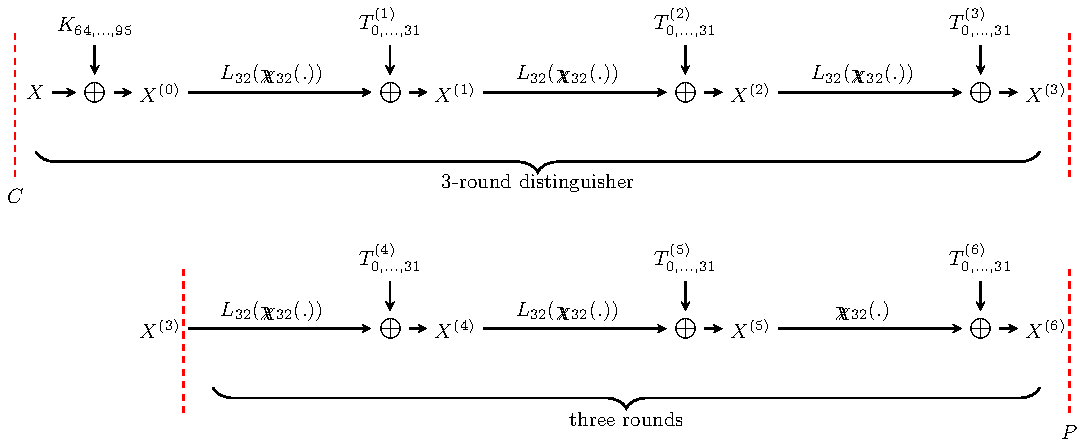
\includegraphics[width=1\textwidth]{figures/chilow_fig_6R.pdf} % image file name
	\caption{Attack on 6-round CHILOW-(32+$\tau$).}
	\label{fig:6R_attack} % your defined label.
\end{figure*}







%%%%%%%%%%%%%%%%%%%%%%%%%%%%%%%%%%%%%%%%%%%%%%%%%%%%%%%%%%%%%%%%%%%%%%%%%%%%%%%%%%%%%%%%%%%%%%%%%%

\begin{algorithm}
\caption{Key-Recovery Attack on 6-round CHILOW(32+$\tau$)}\label{alg}
\LinesNumbered
% This is to hide end and get the last vertical line straight
\SetKwBlock{Begin}{Begin}{}
\SetAlgoLined
  \textbf{Input:} { Three distinct sets of $2^4$ pairs of $(P,C)$ s.t. $C_{0,...,20,22,24,26,28,...,31}$ is constant in each set. }\\
\textbf{Output:} A set of candidates $\mathcal{K}$ for master key.\\
$\mathcal{K}=\emptyset$\\
$\mathcal{T}=\emptyset$\\{}
\ForAll(\tcp*[f]{$1^{st}$ phase}){$T^{(6)}_{0,...,31}||T^{(5)}_{0,...,31}||T^{(4)}_{0,...,31}$} {
             $PAR=0$\\
             \ForAll{$2^3$ pairs of $(P,C)$ in the $1^{st}$ input set s.t. $C_{0,...,20,22,24,26,...,31}$ is constant} {
                $X^{(3)}=\chi\!\!\!\chi_{32}^{-1}(L_{32}^{-1}(\chi\!\!\!\chi_{32}^{-1}(L_{32}^{-1}(\chi\!\!\!\chi_{32}^{-1}(P\oplus T^{(6)}_{0,...,31}) \oplus T^{(5)}_{0,...,31}))\oplus T^{(4)}_{0,...,31}))$\\
                $PAR=PAR \oplus X^{(3)}$\\
            }
            \If{$PAR_{2,3,14,25,26}\neq 0$}{\textbf{break}}
            $PAR=0$\\
             \ForAll{$(P,C)$ in the $1^{st}$ input set} {
                $X^{(3)}=\chi\!\!\!\chi_{32}^{-1}(L_{32}^{-1}(\chi\!\!\!\chi_{32}^{-1}(L_{32}^{-1}(\chi\!\!\!\chi_{32}^{-1}(P\oplus T^{(6)}_{0,...,31}) \oplus T^{(5)}_{0,...,31}))\oplus T^{(4)}_{0,...,31}))$\\
                $PAR=PAR \oplus X^{(3)}$\\}
                \If{$PAR \neq 0$}{\textbf{break}}
            $PAR=0$\\
             \ForAll{$(P,C)$ in the $2^{nd}$ input set} {
                $X^{(3)}=\chi\!\!\!\chi_{32}^{-1}(L_{32}^{-1}(\chi\!\!\!\chi_{32}^{-1}(L_{32}^{-1}(\chi\!\!\!\chi_{32}^{-1}(P\oplus T^{(6)}_{0,...,31}) \oplus T^{(5)}_{0,...,31}))\oplus T^{(4)}_{0,...,31}))$\\
                $PAR=PAR \oplus X^{(3)}$\\}
                \If{$PAR \neq 0$}{\textbf{break}}
            $PAR=0$\\
             \ForAll{$(P,C)$ in the $3^{rd}$ input set} {
                $X^{(3)}=\chi\!\!\!\chi_{32}^{-1}(L_{32}^{-1}(\chi\!\!\!\chi_{32}^{-1}(L_{32}^{-1}(\chi\!\!\!\chi_{32}^{-1}(P\oplus T^{(6)}_{0,...,31}) \oplus T^{(5)}_{0,...,31}))\oplus T^{(4)}_{0,...,31}))$\\
                $PAR=PAR \oplus X^{(3)}$\\}
                \If{$PAR=0$}{ $\mathcal{T}=\mathcal{T} \cup \{T^{(6)}_{0,...,31}||T^{(5)}_{0,...,31}||T^{(4)}_{0,...,31}\}$}
}
$\mathcal{T'}=\emptyset$\\{}
\ForAll(\tcp*[f]{$2^{nd}$ phase}){$T^{(3)}_{0,...,31}$} {
    \ForAll{$T^{(6)}_{0,...,31}||T^{(5)}_{0,...,31}||T^{(4)}_{0,...,31}\in \mathcal{T}$}{
             $PAR=0$\\
             \For{$2^2$ pairs of $(P,C)$ in the $1^{st}$ input set s.t. $C_{0,...,20,22,24,...,31}$ is constant} {
                $X^{(2)}=\chi\!\!\!\chi_{32}^{-1}(\chi\!\!\!\chi_{32}^{-1}(L_{32}^{-1}(\chi\!\!\!\chi_{32}^{-1}(L_{32}^{-1}(\chi\!\!\!\chi_{32}^{-1}(P\oplus T^{(6)}_{0,...,31}) \oplus T^{(5)}_{0,...,31}))\oplus T^{(4)}_{0,...,31}))\oplus T^{(3)}_{0,...,31}))$\\
                $PAR=PAR \oplus X^{(2)}$\\
            }
            \If{$PAR=0$}{
                $\mathcal{T'}=\mathcal{T'} \cup \{T^{(6)}_{0,...,31}||T^{(5)}_{0,...,31}||T^{(4)}_{0,...,31}||T^{(3)}_{0,...,31}\}$}
        }
    }
\end{algorithm}


\SetNlSty{texttt}{(}{)}
\begin{algorithm}
%\caption{Key-Recovery Attack on 6-round CHILOW(32+$\tau$)-continued}\label{alg}
  \LinesNumbered
\setcounter{AlgoLine}{40}
% This is to restore vline mode if you did not take the package as \usepackage[linesnumbered,ruled,vlined]{algorithm2e}
  \SetAlgoVlined
%This is to hide Begin keyword

$\mathcal{T}=\emptyset$\\{}
\ForAll(\tcp*[f]{$3^{rd}$ phase}){$T^{(2)}_{0,...,31}||T^{(1)}_{0,...,31}||K_{64,...,95}$} {
    \ForAll{$T^{(6)}_{0,...,31}||T^{(5)}_{0,...,31}||T^{(4)}_{0,...,31}||T^{(3)}_{0,...,31}\in \mathcal{T'}$}{
             \For{3 distinct pairs of $(P_i,C_i)$ in the $1^{st}$ input set} {
                \If{$P_1=D_{32}(C_1)$ and $P_2=D_{32}(C_2)$ and $P_3=D_{32}(C_3)$}{
                $\mathcal{T}=\mathcal{T} \cup \{T^{(6)}_{0,...,31}||T^{(5)}_{0,...,31}||T^{(4)}_{0,...,31}||T^{(3)}_{0,...,31}||T^{(2)}_{0,...,31}||T^{(1)}_{0,...,31}||K_{64,...,95}\}$}
        }
        }
    }
$\mathcal{T'}=\emptyset$\\{}
\ForAll(\tcp*[f]{$4^{th}$ phase}){$T^{(1)}_{32,...,63}$} {
    \ForAll{$T^{(1)}_{0,...,31}\in \mathcal{T}$}{
        $K_{0,...,63}=\chi\!\!\!\chi_{64}^{-1}(L_{64}^{-1}(T^{(1)}))\oplus T$
        $\mathcal{T'}=\mathcal{T'} \cup \{T^{(6)}_{0,...,31}||T^{(5)}_{0,...,31}||T^{(4)}_{0,...,31}||T^{(3)}_{0,...,31}||T^{(2)}_{0,...,31}||T^{(1)}_{0,...,31}||K_{0,...,95}\}$
    }
}
\ForAll{$K_{96,...,127}$} {
    \ForAll{$T^{(6)}_{0,...,31}||T^{(5)}_{0,...,31}||T^{(4)}_{0,...,31}||T^{(3)}_{0,...,31}||T^{(2)}_{0,...,31}||T^{(1)}_{0,...,31}||K_{0,...,95}\in \mathcal{T}$}{
        $T'^{(1)}=L_{64}(\chi\!\!\!\chi_{64} (T\oplus K_{0,...,63})$\\
        $T'^{(2)}=L_{64}(\chi\!\!\!\chi_{64} (T'^{(1)}\oplus K_{0,...,63}^{(1)})$\\
        \If{$T'^{(2)}_{0,...,31}\neq T^{(2)}_{0,...,31}$}{\textbf{break}}
        $T'^{(3)}=L_{64}(\chi\!\!\!\chi_{64} (T'^{(2)}\oplus K_{0,...,63}^{(2)})$\\
        \If{$T'^{(3)}_{0,...,31}\neq T^{(3)}_{0,...,31}$}{\textbf{break}}
        $T'^{(4)}=L_{64}(\chi\!\!\!\chi_{64} (T'^{(3)}\oplus K_{0,...,63}^{(3)})$\\
        \If{$T'^{(4)}_{0,...,31}\neq T^{(4)}_{0,...,31}$}{\textbf{break}}
        $T'^{(5)}=L_{64}(\chi\!\!\!\chi_{64} (T'^{(4)}\oplus K_{0,...,63}^{(4)})$\\
        \If{$T'^{(5)}_{0,...,31}\neq T^{(5)}_{0,...,31}$}{\textbf{break}}
        $T'^{(6)}=L_{64}(\chi\!\!\!\chi_{64} (T'^{(5)}\oplus K_{0,...,63}^{(5)})$\\
        \If{$T'^{(6)}_{0,...,31}\neq T^{(6)}_{0,...,31}$}{\textbf{break}}
        $\mathcal{K}=\mathcal{K} \cup K$
    }
}

\Return{$\mathcal{K}$}  
\end{algorithm}

%%% CONCLUSION %%%%%%%%%%%%%%%%%%%%%%%%%%%%%%%%%%%%%%%%%%%%%%%%%%%%%%%%%
\section{Conclusion}\label{sec:conclusion}

...


\ifspringer
  \bibliographystyle{splncs04}
\else
  \bibliographystyle{alphaurl}
\fi
\iffinal
  \bibliography{main}
\else
  \bibliography{\jobname}
\fi


\iffinal\else
% appendix/auxiliary material here
% ...
\fi


% move to main.bib for final version!
\begin{filecontents*}[overwrite]{\jobname.bib}

@article{DBLP:journals/joc/DobraunigEMS21,
  author    = {Christoph Dobraunig and
               Maria Eichlseder and
               Florian Mendel and
               Martin Schl{\"{a}}ffer},
  title     = {{Ascon} v1.2: Lightweight Authenticated Encryption and Hashing},
  journal   = {J. Cryptol.},
  volume    = {34},
  number    = {3},
  pages     = {33},
  year      = {2021},
  doi       = {10.1007/s00145-021-09398-9},
}

\end{filecontents*}

\end{document}
